\section{Residual core: details, noise models and techniques}\label{sec:core}
This appendix collects the details behind \cref{sec:reduction,sec:sota}: exact pruning, the map of the core, the generic preparation with measurement-based uncomputation, a hybrid with a cheaper objective layer, the noise models, and the techniques tried (including negative results). All circuits are compiled to the \texttt{ibm\_fez} topology or simulated; nothing was executed on a device.

\paragraph{Exact pruning of the layer.} The classical reduction fixes an interface (the long and short counts of every period and sector). Given the interface, every variable that takes the same value in all feasible strings of its block is known, so it is removed from the objective (terms with a known zero vanish, terms with a known one become linear); blocks with a single feasible string need no mixer; a block with no long (or no short) position uses a two-qubit swap rotation instead of the four-qubit pair exchange; and a constraint gauge rewrites couplings with the constant group counts. All steps leave the state on the feasible set unchanged (\cref{tab:core_prune}; checked against a dense simulation for $n\le16$ and by two statevector simulations at $n=24$). They cut the compiled layer by $4$--$8\times$ (at $n=24$ from $1131$ to $259$--$262$ CZ gates, with the median estimated success probability going from $0.01$ to $0.36$--$0.38$). Dropping weak couplings (approximate) adds little beyond the exact steps for $n\le16$. \emph{The reduction is large because the interface fixes most variables}: on average only $2.5$, $6.0$, $6.9$ and $11.1$ of the $8$, $12$, $16$ and $24$ variables remain free. The quantum problem that is left is small, and this must be read together with every executability claim of \cref{sec:large}.

\begin{table}[t]
\centering\footnotesize\setlength{\tabcolsep}{4pt}
\caption{\orig{compiled counts (CZ for this compiler and topology) and ESP (noise model); nothing executed} Exact pruning of one QAOA layer ($p=1$) for the multi-constraint case, averaged over interface tuples sampled with their weight (8--12 per size), compiled to the \texttt{ibm\_fez} topology (best of three seeds; nothing executed). S0: symmetric preparation, pair-exchange mixers, full objective. S2: variables fixed by the interface eliminated from the objective, blocks with a single feasible string get no mixer, two-qubit swap rotations when a block has no long or no short position. S3: S2 plus a constraint gauge that rewrites couplings with the constant group counts. All three give the same state on the feasible set (defect $\le10^{-14}$ against a dense simulation for $n\le16$ and $1.3\cdot10^{-14}$ by two statevector simulations at $n=24$). The reduction is large because the interface fixes most variables: the last column of the left block is the mean number of qubits that remain free.}\label{tab:core_prune}
\begin{tabular}{rrrrrrrr}
\toprule
$n$ & free & \multicolumn{3}{c}{CZ (mean)} & \multicolumn{3}{c}{ESP (median)}\\ & qubits & S0 & S2 & S3 & S0 & S2 & S3\\
\midrule
8 & 2.5 & 178 & 27 & 22 & 0.57 & 0.93 & 0.93\\
12 & 6.0 & 418 & 78 & 51 & 0.25 & 0.81 & 0.86\\
16 & 6.9 & 506 & 88 & 91 & 0.17 & 0.74 & 0.72\\
24 & 11.1 & 1131 & 262 & 259 & 0.01 & 0.36 & 0.38\\
\bottomrule
\end{tabular}
\end{table}




\paragraph{Gate counts of the four methods on the same core.} With the same classically reduced, dense objective, Fourier-LCU in its single-basis form replaces each count constraint by one layer of single-qubit $R_z$ gates, and unbalanced penalisation adds penalty terms that fall on pairs the dense objective already couples; both therefore cost no more two-qubit gates than the objective itself. Our QAOA layer adds the preparation and the mixers, which is $77\%$ to $14\%$ of the objective's gates as the core grows from $48$ to $512$ variables (before routing; \path{results/four_methods.json}). After routing to the heavy-hex lattice our layer has $\approx2\times$ the CZ gates ($1.9$--$2.5\times$ on average over six cores of $16$--$64$ qubits) and $2.6$--$3.7\times$ the depth of the baselines. Hence \emph{per layer our circuit is more expensive than both}; what it buys is that every sample is feasible by construction. For amplitude amplification only our construction applies (the other two are QAOA variants); one iteration costs $645$--$34{,}000$ CZ for cores of $23$--$326$ free qubits (ancilla-free reflection, not routed), and a Grover search over all $2^f$ strings with a feasibility oracle needs $2^{(f-\log_2|F|)/2}$ times more iterations, from $2^{7}$ to $2^{95}$ in the families above.


\paragraph{Note on the cores of \cref{tab:core_cases}.} The interface tuple is drawn at random, so cores from different experiments can differ in the tuple while keeping the size (for $n=100$, the experiments after that table use a second tuple with the same $20$ free qubits and $10^4$ feasible strings), and the best-of-seeds compilation is rerun ($473$ against $464$ CZ at $n=64$). Values are therefore comparable only within one table or paragraph.
\paragraph{The same layer without the Dicke shortcut.} The symmetric lowering (Dicke states and controlled swaps) exists only for interchangeable units and is not specific to our construction. \Cref{tab:core_generic} replaces it by the generic automaton preparation $A_q$ for any constraint set, with its registers uncomputed. The preparation alone grows from $28$, $215$ and $289$ to $795$, $3056$ and $4791$ CZ gates ($14$--$28\times$) and from $16$, $20$ and $30$ qubits to $58$, $90$ and $132$. \emph{Measurement-based uncomputation} (\path{negsearch/mbu.py}) measures each register qubit in the $X$ basis and removes the phase $(-1)^r$ with the CZ gates that define it, without Toffoli gates; it is exact (fidelity $1$ on all outcomes of small blocks) and cuts the one-hot preparation by $38\%$ and $23\%$ in expected CZ gates and by $1.3$--$2\times$ in qubits, but against the binary register it wins only at $n=100$ and $192$ ($1841$ against $3056$ and $3037$ against $4791$ CZ) and loses at $n=64$. One layer on it takes $2.0$, $2.9$ and $4.9$ thousand CZ gates (worst case) against $464$, $581$ and $923$ for the symmetric lowering, with an estimated success probability of zero at this precision. \emph{So the part specific to us, the automaton for arbitrary constraints, does not run on today's devices at these sizes, even with measurement-based uncomputation; what runs is the symmetric special case.}
\begin{table*}[t]
\centering\footnotesize\setlength{\tabcolsep}{4pt}
\caption{\orig{compiled counts; nothing executed} Our construction with and without the symmetric (Dicke-based) lowering, on the three cores. Entries: symmetric lowering / generic automaton preparation $A_q$ with binary registers uncomputed in reverse / generic one-hot register with measurement-based uncomputation and one pool of reused register qubits. ``qubits'' are those of the preparation alone; CZ are for the preparation alone and for one QAOA layer (same objective and mixers; for the measurement-based version the layer uses the worst case, all corrections applied, and the preparation column the expected value, half of the corrections). Compiled to \texttt{ibm\_fez} (best of three seeds). The one-hot register with reverse uncomputation needs $90$, $119$ and $179$ qubits (it does not fit at $n=192$) and $1611$, $2385$ CZ at $n=64$, $100$.}\label{tab:core_generic}
\begin{tabular}{rrrrr}
\toprule
$n$ & free & qubits (prep) & CZ (prep) & CZ (layer)\\
\midrule
64 & 16 & 16 / 58 / 60 & 28 / 795 / 1002 & 464 / 1543 / 2025\\
100 & 20 & 20 / 90 / 61 & 215 / 3056 / 1841 & 581 / 3704 / 2886\\
192 & 30 & 30 / 132 / 88 & 289 / 4791 / 3037 & 923 / 6375 / 4937\\
\bottomrule
\end{tabular}
\end{table*}


\paragraph{Combining with other methods.} A diagonal layer of any kind keeps the support, so any approximation of the objective layer keeps feasibility and only affects quality (\path{experiments/hybrid_nocost.py}, \path{experiments/hybrid_quality.py}). Without the two-qubit objective layer, our preparation and mixers compile to $66$, $260$ and $357$ CZ gates with ESP $0.80$, $0.41$ and $0.24$, against $0.20$, $0.15$ and $0.04$ with it. A single-qubit mean-field layer, $g_i=h_i+\sum_jJ_{ij}\langle x_j\rangle_F$, as the cheapest stand-in for a Fourier-type decomposition keeps the ideal quality ($0.741$, $0.700$, $0.622$ against $0.731$, $0.677$, $0.599$ with the full layer, and $0.584$, $0.483$, $0.439$ for uniform sampling of $F$). It is not the Fourier-LCU method, which has its own sampling overhead, and the mean-field problem is easy for a classical computer, so a quantum layer on top of it adds a benefit only if it improves the classical solution of that linearisation, which these experiments do not test. A classical solution can also bias the amplitudes of the preparation, which is the experiment of \cref{tab:tilted_prep}; a threshold for amplification from a classical solution in the fault-tolerant regime was not run.
\paragraph{Which noise model.} We use three levels. (i)~\emph{ESP}, the product of one minus the error of every gate of the compiled circuit (error rates of the backend's calibration), as a first filter. (ii)~A \emph{global depolarising model}: the output is $\mathrm{ESP}\cdot P_\mathrm{ideal}+(1-\mathrm{ESP})\cdot\mathrm{uniform}$, which predicts the fraction of feasible shots as $\mathrm{ESP}\,P_\mathrm{ideal}^{\mathrm{feas}}+(1-\mathrm{ESP})|F|/2^f$. (iii)~A \emph{gate-level noisy simulation} (Aer with the noise model of \texttt{FakeFez}: gate errors, thermal relaxation, readout), possible up to about $20$ qubits. \Cref{tab:core_noise} compares (ii) and (iii) on the $16$-qubit core: the model is conservative, giving $18.1\%$ feasible shots against $21.8\pm1.7\%$ simulated for our layer and $0.8\%$ against $2.0\pm0.6\%$ for the single-basis LCU-like layer; the duration of the circuit is $0.18\,T_2$, so relaxation is not the dominant error. We therefore use the ESP model as a lower bound and the gate-level simulation as the check, and the calibration of the day of the run would replace both. None of this is a measurement.

\begin{table*}[t]
\centering\footnotesize\setlength{\tabcolsep}{4pt}
\caption{\orig{depolarising model checked against a gate-level noisy simulation; no hardware} The global-depolarising model against a gate-level noisy simulation (Aer, noise model of \texttt{FakeFez}: gate errors, thermal relaxation, readout; $600$ shots) on the $n=64$ case with $16$ free qubits. Model: feasible fraction $=\mathrm{ESP}\cdot P_\mathrm{ideal}+(1-\mathrm{ESP})|F|/2^f$. Quality after post-selecting the feasible shots is compared with its ideal value. The LCU-like row has untrained angles and is only a check of the noise model, not of that method.}\label{tab:core_noise}
\begin{tabular}{lrrrrrrr}
\toprule
circuit & CZ & ESP & ideal feas.\,\% & model\,\% & simulated\,\% & ideal qual. & post-sel. qual.\\
\midrule
ours (QAOA layer) & 450 & 0.180 & 100.0 & 18.1 & 21.8$\pm$1.7 & 0.717 & 0.713\\
single-basis LCU-like layer & 371 & 0.245 & 3.0 & 0.8 & 2.0$\pm$0.6 & 0.532 & 0.540\\
\bottomrule
\end{tabular}
\end{table*}


\paragraph{Techniques, and what they buy.} \emph{Classical reduction and exact pruning} lower the CZ count by $4$--$8\times$ (\cref{tab:core_prune}) at no cost. \emph{Reflection with ancillas:} a Toffoli V-chain for the reflection about $|0\rangle$ cuts one amplification iteration by $6.8$--$10.7\times$ for $f-3$ more qubits (the dirty-ancilla and recursive variants are worse: $1.5$ and $2.2$ thousand CZ at $f=30$ against $1.3$). \emph{Fusion (negative results;} \path{experiments/fused_mixer.py}, \path{experiments/swap_network_objective.py}\emph{):} absorbing the $ZZ$ phase into the swap rotation, $e^{-i\beta\,\mathrm{SWAP}}e^{-i\gamma cZZ}=R_{XX}R_{YY}R_{ZZ}$, is exact ($5\cdot10^{-15}$) but saves less than the transpiler's variance ($479$, $606$, $1040$ CZ against $449$, $619$, $990$), because the mixers are only $10$--$25\%$ of the layer; the brick-wall order does not lower the count but does not hurt the QAOA either (ideal quality $0.731$, $0.677$, $0.599$ against $0.718$, $0.663$, $0.591$ for the sequential path); a line swap network for the objective gives $361$ CZ against $382$ on the dense $16$-qubit core but is much worse on sparse cores ($565$ against $296$ at $20$ qubits); and the preparation cannot absorb the cost layer. \emph{Layout and routing selection by ESP} (best of several transpiler seeds) is used for every compiled circuit. \emph{Post-selection on feasibility} is free for a feasible-by-construction circuit and turns noise into a loss of shots by $1/\mathrm{ESP}$ ($5$, $15$ and $27$ for the three cases) instead of a distortion: on the $16$-qubit core the quality after post-selection is $0.713$ against $0.717$ ideal (\cref{tab:core_noise}), but errors that map a feasible string to another feasible string are not detected. Probabilistic error cancellation would need a sampling overhead of order $\exp(4\varepsilon N_\mathrm{CZ})$ with $\varepsilon\approx0.0035$ ($7\cdot10^{2}$ at $473$ CZ, $4\cdot10^{5}$ at $923$) and zero-noise extrapolation triples the circuit; neither, nor dynamical decoupling, twirling or readout mitigation, was applied.
\paragraph{Depth and gates on today's hardware.} A $p=1$ layer on a core of $16$, $20$ and $30$ free qubits compiles to $473$, $669$ and $923$ CZ gates, depth $541$, $607$ and $586$, and an estimated success probability of $0.19$, $0.066$ and $0.037$; the effective error per CZ over the nine compiled circuits of \cref{tab:core_cases} is $0.0035$--$0.0041$, so $\mathrm{ESP}\approx e^{-0.0035\,N_\mathrm{CZ}}$, and one free qubit costs about $31$ CZ gates. A layer with ESP $\ge0.3$ allows about $11$ free qubits and one with ESP $\ge0.1$ about $21$; an error per CZ three times smaller would allow $33$ and $63$, ten times smaller $110$ and $211$, under the same linear growth; with $p>1$ the numbers divide by $p$. Shots to see the optimum once: $125$, $3.8\cdot10^{3}$ and $1.3\cdot10^{6}$ for our layer against $64$, $5.0\cdot10^{3}$ and $3.0\cdot10^{5}$ for uniform sampling of the feasible set, which is a classical routine. Against the uniform-start baselines under the same depolarising model our layer gives $0.80\%$ probability of the optimum per shot against $0.23\%$ (Fourier-LCU) and $0.15\%$ (unbalanced) at $16$ free qubits, and $0.026\%$ against $0.006\%$ and $0.002\%$ at $20$. Amplitude amplification does not run in full: an iteration with an ancilla-free reflection costs $3.5$, $6.3$ and $8.7$ thousand CZ gates for the three cores, and a Toffoli V-chain cuts it to $323$, $800$ and $1279$ CZ ($31$, $40$ and $64$ qubits, ESP per iteration $0.31$, $0.034$ and $0.003$); the $6$, $56$ and $433$ iterations needed give an overall ESP of about $8\cdot10^{-4}$ for the first core and negligible for the others, so its use is fault tolerant (\cref{tab:large_grover_ft}).
\paragraph{Summary.} The conclusions drawn from this appendix are stated in \cref{sec:sota}: the theory holds in every case checked, the classical reduction is exact and large, our layer is feasible at every shot in ideal simulation and is predicted to run on cores of up to about $16$--$20$ free qubits, the generic automaton is not predicted to run at these sizes, and amplification is a fault-tolerant use.

\paragraph{Stronger baselines (experiment).} \orig{exact dense simulation, compiled counts, depolarising model; nothing executed} The first baselines of this appendix start from the uniform state, which is weaker than what the cited papers use. We therefore repeated the comparison on the residual core with all baselines starting from the warm-started product state $\mathrm{RY}(2\arcsin\sqrt{k/m})$ per qubit, with $12$ random restarts of the angles at $p=1$ (\path{experiments/baselines_strong.py}, \path{experiments/make_baselines_table.py}, \cref{tab:core_baselines}): a single-basis Fourier-LCU variant with trained phases per count group, the unbalanced penalty with the best of three $(\ell_1,\ell_2)$ pairs and exclusivity phases, and an XY mixer inside count groups. The advantage of our construction narrows: all samples remain feasible and no penalty weight is tuned, but the per-shot gain in the probability of the optimum is modest ($1.2$--$3.3\times$ at $16$ free qubits) and erratic at $20$ free qubits, where four instances were run ($4$ or $8$ restarts) and our layer is best in three, by $7$ to $22$ times, and $2.5$ times worse in one. The cores are small ($|F|=64$ and $10^4$), the Fourier-LCU variant is the single-basis form without sampling or CVaR, and results at $p=2$ are in the result files. The single-basis form is the favourable one for that method: in the Fourier-LCU paper's own $12$-node table the single LCU basis gave the highest probability of the optimum ($0.0317$, against $0.0024$ for the re-optimised sampled version, whose sampling cost is $\Gamma=\|c\|_1^2\le\sqrt{n+1}$ per constraint), so we did not implement the sampled version. These numbers should be read as a check against overstating, not as a benchmark.

\begin{figure*}[t]\centering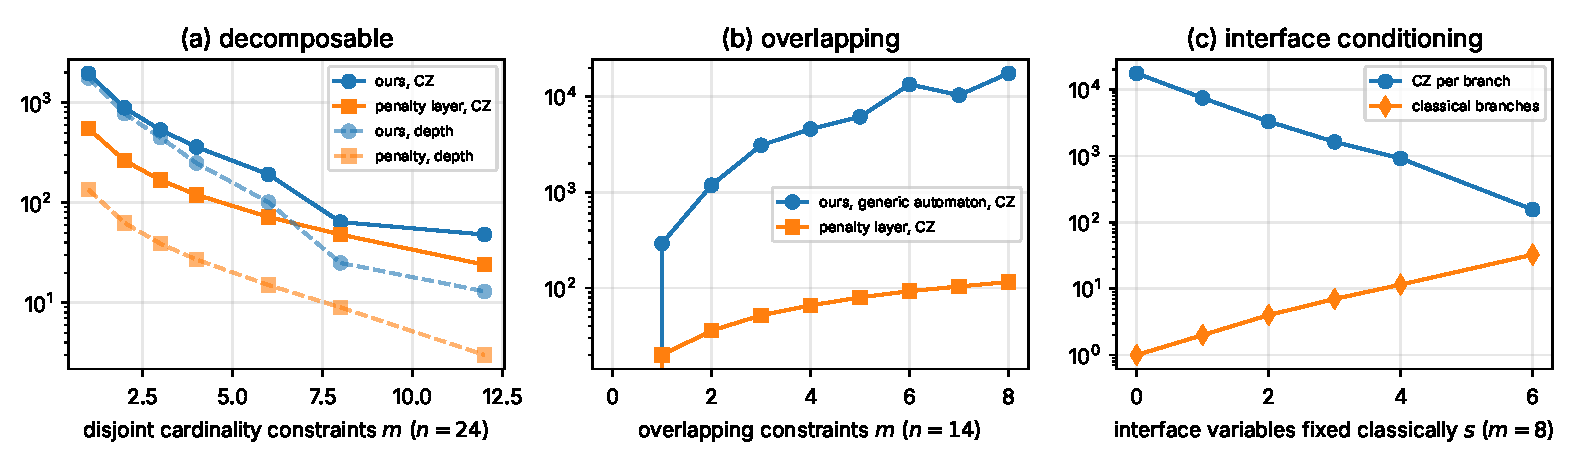
\includegraphics[width=\textwidth]{figures/constraint_scaling.pdf}\caption{\orig{exact enumeration, compiled counts, all-to-all; no noise} Cost of the feasibility block against the number of constraints. (a)~$n=24$ split in $m$ disjoint groups with exactly half of each group on: our block (Dicke per group) and the constraint phase layer of a penalty or unbalanced circuit. (b)~Random overlapping constraints (sum over five of $14$ variables at most two), generic automaton circuit with the best of six variable orders, mean of two instances. (c)~Same constraints, $m=8$: fixing $s$ variables classically lowers the CZ count per branch and increases the number of branches.}\label{fig:constraint_scaling}\end{figure*}

\paragraph{Optimising the Dicke block and the swap chain.} \orig{compiled counts; states checked against the exact one} Every block preparation starts with Dicke states, and with Qiskit's generic controlled gates they cost much more than necessary (\path{negsearch/dicke_opt.py}, \path{experiments/dicke_optimised.py}, \cref{tab:dicke_opt}). Three changes keep the state exactly (fidelity $1$ for every $n\le14$ and $k$). (i)~The doubly controlled RY as two rounds of RY, CX, RY, CX with angles $\pm\theta/4$ ($X\,\mathrm{RY}(\varphi)X=\mathrm{RY}(-\varphi)$ makes the angles add only when both controls are on): $4$ CX, which lowers the count by $32$--$40\%$. (ii)~Since the block acts only on a subspace, a least-squares fit of the whole circuit to the exact state with a three-CX template gave a closed form with $3$ CX (controls $a$, $b$, target $t$): \begin{equation*}\mathrm{RY}_t(\tfrac{\pi}{2}-\tfrac{\theta}{4})\,\mathrm{CX}_{bt}\,\mathrm{RY}_t(\tfrac{\theta}{4})\,\mathrm{CX}_{at}\,\mathrm{RY}_t(-\tfrac{\theta}{4})\,\mathrm{CX}_{bt}\,\mathrm{RY}_t(\tfrac{\theta}{4}-\tfrac{\pi}{2}),\end{equation*}verified for $n\le14$. (iii)~The decompression chain is pruned to the range that can hold a nonzero qubit, and the species with the shorter chain is the control. For a Dicke block of $12$ qubits and $6$ ones, $698\to387$ routed CZ ($-45\%$); the whole preparation of a block drops by $20$--$32\%$ ($(12,6,3)$: $917\to624$ logical CZ). The routing overhead, $1.7$--$1.9\times$, comes from the hub qubit that controls every gate of a stage. In the $120$-qubit prediction the effect is small, because its blocks have $5$ units: the preparation goes from $110$ to $96$ CZ and our light layer from $21\%$ to $22\%$ feasible shots per block, still below the unbalanced baseline ($28\%$). \emph{Negative results on the controlled-swap chain, which is $50$--$60\%$ of the preparation:} no gate cheaper than the controlled swap ($8$ CX, $7$ after optimisation) exists among classical CX and Toffoli circuits of up to five gates even with the don't-care inputs of the pruned chain; a phase-exact numerical resynthesis with up to three CX finds no exact solution (four and more did not finish; \path{experiments/cswap_resynth.py}); a three-symbol generalisation of the Dicke ladder, a network of adjacent exchanges $e^{i\theta\,\mathrm{SWAP}}$ of two units, keeps the support but its gate costs $18$ CX and it needs $18$, $28$, $74$ and $270$ exchanges for $(m,l,s)=(5,2,2)$, $(6,3,2)$, $(8,3,3)$, $(12,4,4)$ against $95$, $138$, $277$ and $666$ CX for the whole optimised preparation, i.e. $3$--$7\times$ more (\path{experiments/three_symbol_exchange.py}). A relative-phase Toffoli inside each controlled swap ($5$ CX instead of $7$) keeps the support and the magnitudes and changes the phases in multiples of $\pi/2$, lowering the preparation to $43$, $77$ and $114$ CX for $(4,2,1)$, $(5,2,2)$, $(6,3,2)$ (from $53$, $95$, $138$), but the quality of our $p=1$ layer, retrained on the actual circuit for the twelve blocks, falls from $0.669$ and $0.715$ to $0.649$ and $0.697$ (\path{experiments/retrain_relphase.py}); it is off by default (\texttt{NS\_REL\_PHASE=1}).

\begin{table*}[t]\centering\scriptsize\setlength{\tabcolsep}{3pt}
\caption{\orig{compiled counts; exact state checked for $n\le12$; nothing executed} Dicke block $|D^n_k\rangle$: CZ count and two-qubit depth, logical (all-to-all) and routed on the \texttt{ibm\_fez} coupling map (best of $10$ transpiler seeds; $6$ for $n\ge16$). ref: generic controlled gates; 4cx: hand-decomposed doubly controlled RY; 3cx: that gate with $3$ CX, exact on the states the block produces.}\label{tab:dicke_opt}
\begin{tabular}{lrrrrrr}\toprule
$(n,k)$ & logical ref & logical 3cx & routed ref & routed 4cx & routed 3cx & 2q depth ref $\to$ 3cx\\\midrule
$(6,3)$ & 73 & 45 & 116 & 65 & 58 & 110$\to$55\\
$(8,4)$ & 149 & 89 & 238 & 152 & 139 & 223$\to$119\\
$(10,5)$ & 252 & 148 & 432 & 277 & 249 & 383$\to$210\\
$(12,6)$ & 382 & 222 & 698 & 432 & 387 & 524$\to$309\\
$(16,8)$ & 723 & 415 & 1395 & 885 & 845 & 779$\to$568\\
$(24,12)$ & 1729 & 981 & 3471 & 2163 & 2034 & 1394$\to$932\\
\bottomrule\end{tabular}\end{table*}


\paragraph{Can the cost function inform the preparation?} \orig{exact simulation of the circuits; classical information from the block QUBO; no noise; nothing executed} Yes, at no cost in gates. Any state with support $F$ is a valid start, and the Dicke circuit of the preparation reaches a biased state by changing only its rotation angles: a least-squares fit of the angles to the target amplitudes $\sqrt{w(x)}$, $w=\prod_i r_i^{x_i}$ on $F$, reaches zero residual on the cases tried ($(n,k)$ up to $(6,3)$), and the CX count is that of the unbiased circuit (\path{experiments/tilted_prep.py}, \cref{tab:tilted_prep}). On the twelve blocks of the $120$-qubit instance, with the tilt $\exp(-\tau\sum_ig_ix_i)$ built from the mean-field linear field $g$ of the block and $\tau=4$, the preparation alone (the angles of the Dicke blocks, the swap chain unchanged) gives a quality among feasible samples of $0.80$ instead of $0.50$, and a probability of the block optimum of $27\%$ instead of $7\%$; the $p=1$ layer then reaches $0.85$ instead of $0.67$. A Boltzmann tilt, which needs the full cost of every feasible string, reaches $0.96$, but its smallest probability on $F$ is $4\cdot10^{-10}$, so it is an upper bound and the circuit is then a classical solution loaded into a state. Three cautions. First, the information is classical and the blocks are small ($|F|\le30$): they are solvable by enumeration, so this shows what a quantum layer can refine, not an advantage; the tilt strength $\tau$ interpolates between the exploration of the uniform state and loading a classical solution, and the best value here was at the edge of the grid. Second, the baselines profit as much. Giving the three warm-started baselines the marginals of the same tilted distribution as the start of their product state raises their quality at $p=1$ from $0.74$, $0.51$ and $0.73$ to $0.91$, $0.84$ and $0.91$ (Fourier-LCU variant, unbalanced penalty, XY mixer), above our $0.85$, with an ideal feasible fraction of $0.38$, $0.69$ and $0.33$; ours remains $1$, which is the advantage that survives, and after noise the feasible fraction of every circuit is multiplied by its ESP. Third, the angles of the Dicke blocks that realise the tilt were fitted numerically per block; a closed form for the angles from the fugacities is not derived, and the shorts are tilted through the compressed coordinates of the swap chain, so the realised state follows the target only approximately (the quality of the realised state is $0.80$ against $0.81$ of the target).
\begin{table*}[t]\centering\small
\caption{\orig{exact simulation of the logical circuits, $12$ blocks of the $120$-qubit instance; no noise; nothing executed} Cost-informed preparation. Feasible: ideal fraction of feasible samples; quality among feasible samples ($1$ is the best of the block); $P(\mathrm{opt})$: probability of the block optimum at $p=0$. Tilt: product tilt $\exp(-\tau\sum_i g_ix_i)$ with the mean-field field $g$ of the block, $\tau=4$ (edge of the grid), realised by changing only the angles of the Dicke blocks. Boltzmann: $\exp(-\tau c(x))$, an upper bound (its smallest probability on $F$ is $4\cdot10^{-10}$, so the support is exact only in name). Baselines: warm start with $k/m$ (plain) or with the marginals of the tilted distribution (biased), $p=1$.}\label{tab:tilted_prep}
\begin{tabular}{lrrrr}\toprule
preparation / method & feasible & quality $p{=}0$ & quality $p{=}1$ & $P$(opt) $p{=}0$\\\midrule
ours, uniform on $F$ & $1$ & 0.50 & 0.67 & 7\,\%\\
ours, product tilt & $1$ & 0.80 & 0.85 & 27\,\%\\
ours, Boltzmann (upper bound) & $1$ & 0.96 & 0.97 & 69\,\%\\\midrule
Fourier-LCU variant, plain & 0.24 & -- & 0.74 & --\\
Fourier-LCU variant, biased & 0.38 & -- & 0.91 & --\\
unbalanced penalty, plain & 0.59 & -- & 0.51 & --\\
unbalanced penalty, biased & 0.69 & -- & 0.84 & --\\
XY mixer, plain & 0.24 & -- & 0.73 & --\\
XY mixer, biased & 0.33 & -- & 0.91 & --\\
\bottomrule\end{tabular}\end{table*}


